\documentclass{book}
\usepackage[a4paper,top=2.5cm,bottom=2.5cm,left=2.5cm,right=2.5cm]{geometry}
\usepackage{makeidx}
\usepackage{natbib}
\usepackage{graphicx}
\usepackage{multicol}
\usepackage{float}
\usepackage{listings}
\usepackage{color}
\usepackage{ifthen}
\usepackage[table]{xcolor}
\usepackage{textcomp}
\usepackage{alltt}
\usepackage{ifpdf}
\ifpdf
\usepackage[pdftex,
            pagebackref=true,
            colorlinks=true,
            linkcolor=blue,
            unicode
           ]{hyperref}
\else
\usepackage[ps2pdf,
            pagebackref=true,
            colorlinks=true,
            linkcolor=blue,
            unicode
           ]{hyperref}
\usepackage{pspicture}
\fi
\usepackage[utf8]{inputenc}
\usepackage{polski}
\usepackage[T1]{fontenc}

\usepackage{mathptmx}
\usepackage[scaled=.90]{helvet}
\usepackage{courier}
\usepackage{sectsty}
\usepackage{amssymb}
\usepackage[titles]{tocloft}
\usepackage{doxygen}
\lstset{language=C++,inputencoding=utf8,basicstyle=\footnotesize,breaklines=true,breakatwhitespace=true,tabsize=4,numbers=left }
\makeindex
\setcounter{tocdepth}{3}
\renewcommand{\footrulewidth}{0.4pt}
\renewcommand{\familydefault}{\sfdefault}
\hfuzz=15pt
\setlength{\emergencystretch}{15pt}
\hbadness=750
\tolerance=750
\begin{document}
\hypersetup{pageanchor=false,citecolor=blue}
\begin{titlepage}
\vspace*{7cm}
\begin{center}
{\Large My Project }\\
\vspace*{1cm}
{\large Wygenerowano przez Doxygen 1.8.3.1}\\
\vspace*{0.5cm}
{\small N, 25 maj 2014 19:50:21}\\
\end{center}
\end{titlepage}
\clearemptydoublepage
\pagenumbering{roman}
\tableofcontents
\clearemptydoublepage
\pagenumbering{arabic}
\hypersetup{pageanchor=true,citecolor=blue}
\chapter{Dokumentacja zadania lab8}
\label{index}\hypertarget{index}{}\begin{DoxyAuthor}{Autor}
Karolina Morawska 
\end{DoxyAuthor}
\begin{DoxyDate}{Data}
16.\-03.\-2014 
\end{DoxyDate}
\begin{DoxyVersion}{Wersja}
0.\-2 
\end{DoxyVersion}

\chapter{Indeks klas}
\section{Lista klas}
Tutaj znajdują się klasy, struktury, unie i interfejsy wraz z ich krótkimi opisami\-:\begin{DoxyCompactList}
\item\contentsline{section}{\hyperlink{class_n_o_d_e}{N\-O\-D\-E} \\*Modeluje pojęcie \hyperlink{class_n_o_d_e}{N\-O\-D\-E} ,czyli wezel. Klasa modeluje pojęcie node . Jej atrybutem są pola zawierające wskaźnik na lewy ,prawy węzeł i wartość }{\pageref{class_n_o_d_e}}{}
\item\contentsline{section}{\hyperlink{class_para}{Para} \\*Modeluje pojęcie \hyperlink{class_para}{Para}. Klasa modeluje pojęcie para . Jej atrybutem są pola zawierające klucz i wartość }{\pageref{class_para}}{}
\item\contentsline{section}{\hyperlink{classper}{per$<$ K, W $>$} \\*Modeluje pojęcie per. Klasa modeluje pojęcie per(para) . Jej atrybutem są pola zawierające klucz i wartość }{\pageref{classper}}{}
\item\contentsline{section}{\hyperlink{class_tablicaas}{Tablicaas$<$ K, W $>$} \\*Modeluje pojęcie \hyperlink{class_tablicaas}{Tablicaas}. Klasa modeluje pojęcie Tablica asocjacyjna . Jej atrybutem są pola zawierające klucz i wartość }{\pageref{class_tablicaas}}{}
\item\contentsline{section}{\hyperlink{class_tree}{Tree} \\*Modeluje pojęcie \hyperlink{class_para}{Para}. Klasa modeluje pojęcie para . Jej atrybutem jest pole zawierajace root(korzen) }{\pageref{class_tree}}{}
\end{DoxyCompactList}

\chapter{Indeks plików}
\section{Lista plików}
Tutaj znajduje się lista wszystkich plików z ich krótkimi opisami\-:\begin{DoxyCompactList}
\item\contentsline{section}{\hyperlink{czas_8hh}{czas.\-hh} }{\pageref{czas_8hh}}{}
\item\contentsline{section}{\hyperlink{dzialania_8cpp}{dzialania.\-cpp} }{\pageref{dzialania_8cpp}}{}
\item\contentsline{section}{\hyperlink{dzialania_8hh}{dzialania.\-hh} }{\pageref{dzialania_8hh}}{}
\item\contentsline{section}{\hyperlink{kolejka_8hh}{kolejka.\-hh} }{\pageref{kolejka_8hh}}{}
\item\contentsline{section}{\hyperlink{main_8cpp}{main.\-cpp} }{\pageref{main_8cpp}}{}
\item\contentsline{section}{\hyperlink{stos_8hh}{stos.\-hh} }{\pageref{stos_8hh}}{}
\item\contentsline{section}{\hyperlink{stos2_8hh}{stos2.\-hh} }{\pageref{stos2_8hh}}{}
\item\contentsline{section}{\hyperlink{stoslista_8hh}{stoslista.\-hh} }{\pageref{stoslista_8hh}}{}
\item\contentsline{section}{\hyperlink{tablica_8cpp}{tablica.\-cpp} }{\pageref{tablica_8cpp}}{}
\item\contentsline{section}{\hyperlink{tablica_8hh}{tablica.\-hh} }{\pageref{tablica_8hh}}{}
\end{DoxyCompactList}

\chapter{Dokumentacja klas}
\hypertarget{class_graf}{\section{Dokumentacja klasy Graf}
\label{class_graf}\index{Graf@{Graf}}
}


Modeluje pojęcie \hyperlink{class_graf}{Graf}. Klasa modeluje pojęcie graf . Jej atrybutem jest pole zawierajace liste sasedztwa.  




{\ttfamily \#include $<$Graf.\-h$>$}

\subsection*{Metody publiczne}
\begin{DoxyCompactItemize}
\item 
void \hyperlink{class_graf_a924085191a51a6f0afbab7075f26eae3}{Dodajw} (unsigned int wierzcholek)
\begin{DoxyCompactList}\small\item\em Metoda ktora dodaje wierzcholek do grafu. Jej atrybutem jest zmienna typu int o nazwie wierzcholek. \end{DoxyCompactList}\item 
void \hyperlink{class_graf_a462c9d3d65e85fbee8e16bbeb7110803}{Dodajk} (int waga, int w1, int w2)
\begin{DoxyCompactList}\small\item\em Metoda ktora dodaje krawedz do grafu. Jej atrybutem sa zmienne okreslajace wierzcholki przez ktore ma przejsc krawedz i zmienna ktora zawiera wage. \end{DoxyCompactList}\item 
void \hyperlink{class_graf_a989e232821c5f0fa37d993168d56be6f}{Usunk} (int w1, int w2)
\begin{DoxyCompactList}\small\item\em Metoda usuwa krawedz. Jej atrybutem sa dwie zmienne oznaczajace wierzcholki ktorych krawedz ma byc usunieta. \end{DoxyCompactList}\item 
void \hyperlink{class_graf_a9c8c9ffa7ad533e0b5ab71d9addbaab5}{Usunw} (int wierzcholek)
\begin{DoxyCompactList}\small\item\em Metoda usuwa wierzcholek. Jej atrybutem jest zmienna typu int o nazwie wierzcholek. \end{DoxyCompactList}\item 
bool \hyperlink{class_graf_aa153595415bd8bec9bc26bd8fb521492}{Polaczenie} (int w1, int w2)
\begin{DoxyCompactList}\small\item\em Metoda sprawdza czy wystepuje polaczenie miedzy dwoma wierzcholkami. \end{DoxyCompactList}\item 
void \hyperlink{class_graf_a5c5e84172e32e1e0564c931fcb3f7088}{Sasiad} (int w1)
\begin{DoxyCompactList}\small\item\em Metoda sprawdza sasiadow wybranego wierzcholka i wypisuje ich. \end{DoxyCompactList}\item 
void \hyperlink{class_graf_a48ef7dc699b09162388314e67cc6e150}{B\-F\-S} (int wierzcholeks)
\begin{DoxyCompactList}\small\item\em Metoda przeszukiwania wstecz.\-Danymi wejściowymi dla algorytmu jest wierzchołek od którego rozpoczynane jest przeszukiwanie. Początkowo wszystkie wierzchołki kolorowane są na biało, co oznacza, że nie zostały jeszcze odwiedzone.\-Kolejka F\-I\-F\-O Q jest inicjalizowana węzłem startowym, którego kolor ustawiony został na szaro – oznacza to, że węzeł został już odwiedzony, lecz nie zostały odwiedzone węzły do niego sąsiednie. Następnie, pobierany jest pierwszy wierzchołek z kolejki i analizowana jest lista jego sąsiadów. Jeżeli sąsiad jest biały, oznacza to, że nie został jeszcze odwiedzony\-: aktualizowany jest więc jego kolor a następnie jest on dodawany do kolejki. Po przeglądnięciu wszystkich sąsiadów danego węzła kolor węzła bieżącego zmieniany jest na czarny (wszyscy jego sąsiedzi zostali odwiedzeni) i operacja powtarza się dla następnego węzła znajdującego się w kolejce, bądź też (jeżeli kolejka jest pusta) algorytm kończy swoje działanie. \end{DoxyCompactList}\item 
void \hyperlink{class_graf_a8340cd1321426d1a49b5e50f1c7e10f1}{Visit\-Node} (int wierzcholek)
\begin{DoxyCompactList}\small\item\em Pomocnicza metoda przy wyszkukiwaniu w glab, ktora sluzy do odwiedzania wezla.\-Na poczatku zamalowywuje wierzcholek na szaro, nastepnie dla kazdego wierzcholka v na liscie sasiedztwa u sprawdzane jest jezeli v jest bialy odwierz wierzcholek v. \end{DoxyCompactList}\item 
void \hyperlink{class_graf_a8b40e6700dd8f1f71b6b47558c0975a1}{D\-F\-S} ()
\begin{DoxyCompactList}\small\item\em Metoda przeszukiwania w glab.\-Na poczatku dla kazdego wierzcholka u z grafu kolor wierzcholka ustawiany jest na bialy.\-W innym przypadku jezeli wierzcholek jest juz bialy wywolywana jest metoda Visit\-Node. \end{DoxyCompactList}\end{DoxyCompactItemize}
\subsection*{Atrybuty publiczne}
\begin{DoxyCompactItemize}
\item 
vector$<$ int $>$ \hyperlink{class_graf_a8cc46484cf7f96ce274d87829bf10120}{colour}
\begin{DoxyCompactList}\small\item\em Inicjalizuje zmienna typu wektor ktora wykorzystywana jest przy metodach przeszukiwan aby sprawdzic czy dany wierzcholek byl odwiedzany i kolorowany na odpowiedni kolor. \end{DoxyCompactList}\item 
vector$<$ list$<$ \hyperlink{classpara}{para} $>$ $>$ \hyperlink{class_graf_a72ccd052ab732941488da20d198aa82c}{wektor}
\begin{DoxyCompactList}\small\item\em Inicjalizuje zmienna typu lista wektorow . \end{DoxyCompactList}\end{DoxyCompactItemize}


\subsection{Opis szczegółowy}


Definicja w linii 28 pliku Graf.\-h.



\subsection{Dokumentacja funkcji składowych}
\hypertarget{class_graf_a48ef7dc699b09162388314e67cc6e150}{\index{Graf@{Graf}!B\-F\-S@{B\-F\-S}}
\index{B\-F\-S@{B\-F\-S}!Graf@{Graf}}
\subsubsection[{B\-F\-S}]{\setlength{\rightskip}{0pt plus 5cm}void Graf\-::\-B\-F\-S (
\begin{DoxyParamCaption}
\item[{int}]{wierzcholeks}
\end{DoxyParamCaption}
)}}\label{class_graf_a48ef7dc699b09162388314e67cc6e150}


Definicja w linii 56 pliku Graf.\-cpp.

\hypertarget{class_graf_a8b40e6700dd8f1f71b6b47558c0975a1}{\index{Graf@{Graf}!D\-F\-S@{D\-F\-S}}
\index{D\-F\-S@{D\-F\-S}!Graf@{Graf}}
\subsubsection[{D\-F\-S}]{\setlength{\rightskip}{0pt plus 5cm}void Graf\-::\-D\-F\-S (
\begin{DoxyParamCaption}
{}
\end{DoxyParamCaption}
)}}\label{class_graf_a8b40e6700dd8f1f71b6b47558c0975a1}


Definicja w linii 89 pliku Graf.\-cpp.



Oto graf wywołań dla tej funkcji\-:\nopagebreak
\begin{figure}[H]
\begin{center}
\leavevmode
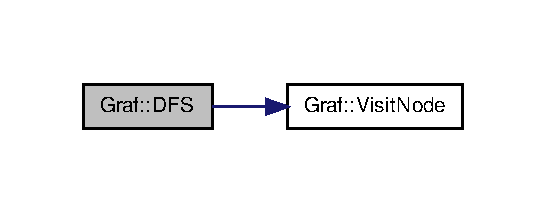
\includegraphics[width=262pt]{class_graf_a8b40e6700dd8f1f71b6b47558c0975a1_cgraph}
\end{center}
\end{figure}


\hypertarget{class_graf_a462c9d3d65e85fbee8e16bbeb7110803}{\index{Graf@{Graf}!Dodajk@{Dodajk}}
\index{Dodajk@{Dodajk}!Graf@{Graf}}
\subsubsection[{Dodajk}]{\setlength{\rightskip}{0pt plus 5cm}void Graf\-::\-Dodajk (
\begin{DoxyParamCaption}
\item[{int}]{waga, }
\item[{int}]{w1, }
\item[{int}]{w2}
\end{DoxyParamCaption}
)}}\label{class_graf_a462c9d3d65e85fbee8e16bbeb7110803}


Definicja w linii 22 pliku Graf.\-cpp.



Oto graf wywołań dla tej funkcji\-:\nopagebreak
\begin{figure}[H]
\begin{center}
\leavevmode
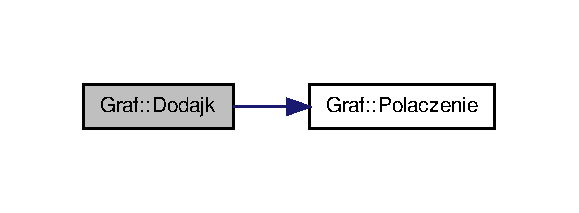
\includegraphics[width=278pt]{class_graf_a462c9d3d65e85fbee8e16bbeb7110803_cgraph}
\end{center}
\end{figure}




Oto graf wywoływań tej funkcji\-:
\nopagebreak
\begin{figure}[H]
\begin{center}
\leavevmode
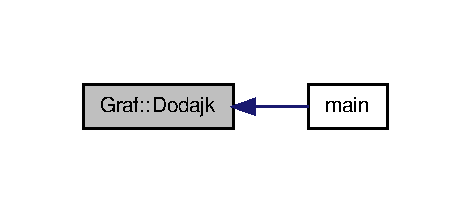
\includegraphics[width=226pt]{class_graf_a462c9d3d65e85fbee8e16bbeb7110803_icgraph}
\end{center}
\end{figure}


\hypertarget{class_graf_a924085191a51a6f0afbab7075f26eae3}{\index{Graf@{Graf}!Dodajw@{Dodajw}}
\index{Dodajw@{Dodajw}!Graf@{Graf}}
\subsubsection[{Dodajw}]{\setlength{\rightskip}{0pt plus 5cm}void Graf\-::\-Dodajw (
\begin{DoxyParamCaption}
\item[{unsigned int}]{wierzcholek}
\end{DoxyParamCaption}
)}}\label{class_graf_a924085191a51a6f0afbab7075f26eae3}


Definicja w linii 14 pliku Graf.\-cpp.



Oto graf wywoływań tej funkcji\-:
\nopagebreak
\begin{figure}[H]
\begin{center}
\leavevmode
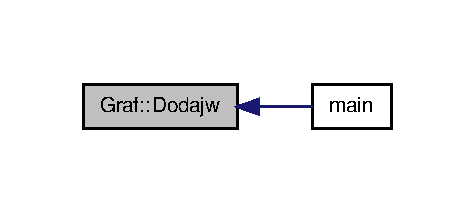
\includegraphics[width=228pt]{class_graf_a924085191a51a6f0afbab7075f26eae3_icgraph}
\end{center}
\end{figure}


\hypertarget{class_graf_aa153595415bd8bec9bc26bd8fb521492}{\index{Graf@{Graf}!Polaczenie@{Polaczenie}}
\index{Polaczenie@{Polaczenie}!Graf@{Graf}}
\subsubsection[{Polaczenie}]{\setlength{\rightskip}{0pt plus 5cm}bool Graf\-::\-Polaczenie (
\begin{DoxyParamCaption}
\item[{int}]{w1, }
\item[{int}]{w2}
\end{DoxyParamCaption}
)}}\label{class_graf_aa153595415bd8bec9bc26bd8fb521492}
\begin{DoxyReturn}{Zwraca}
Zwraca true lub false. 
\end{DoxyReturn}


Definicja w linii 41 pliku Graf.\-cpp.



Oto graf wywoływań tej funkcji\-:
\nopagebreak
\begin{figure}[H]
\begin{center}
\leavevmode
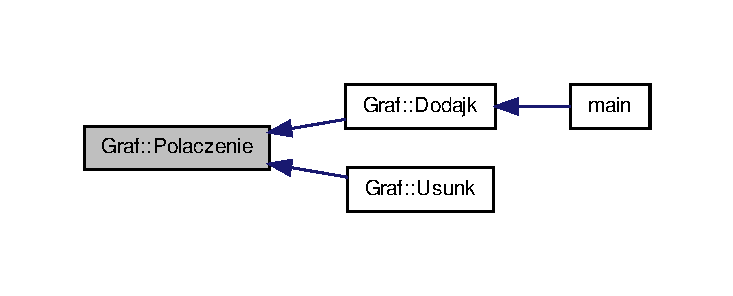
\includegraphics[width=350pt]{class_graf_aa153595415bd8bec9bc26bd8fb521492_icgraph}
\end{center}
\end{figure}


\hypertarget{class_graf_a5c5e84172e32e1e0564c931fcb3f7088}{\index{Graf@{Graf}!Sasiad@{Sasiad}}
\index{Sasiad@{Sasiad}!Graf@{Graf}}
\subsubsection[{Sasiad}]{\setlength{\rightskip}{0pt plus 5cm}void Graf\-::\-Sasiad (
\begin{DoxyParamCaption}
\item[{int}]{w1}
\end{DoxyParamCaption}
)}}\label{class_graf_a5c5e84172e32e1e0564c931fcb3f7088}


Definicja w linii 49 pliku Graf.\-cpp.



Oto graf wywoływań tej funkcji\-:
\nopagebreak
\begin{figure}[H]
\begin{center}
\leavevmode
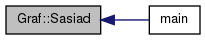
\includegraphics[width=226pt]{class_graf_a5c5e84172e32e1e0564c931fcb3f7088_icgraph}
\end{center}
\end{figure}


\hypertarget{class_graf_a989e232821c5f0fa37d993168d56be6f}{\index{Graf@{Graf}!Usunk@{Usunk}}
\index{Usunk@{Usunk}!Graf@{Graf}}
\subsubsection[{Usunk}]{\setlength{\rightskip}{0pt plus 5cm}void Graf\-::\-Usunk (
\begin{DoxyParamCaption}
\item[{int}]{w1, }
\item[{int}]{w2}
\end{DoxyParamCaption}
)}}\label{class_graf_a989e232821c5f0fa37d993168d56be6f}


Definicja w linii 28 pliku Graf.\-cpp.



Oto graf wywołań dla tej funkcji\-:\nopagebreak
\begin{figure}[H]
\begin{center}
\leavevmode
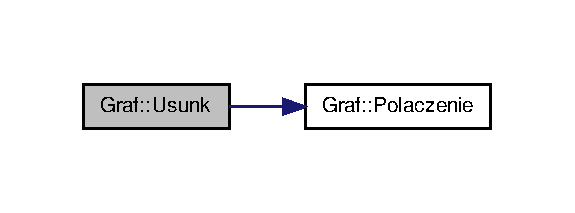
\includegraphics[width=276pt]{class_graf_a989e232821c5f0fa37d993168d56be6f_cgraph}
\end{center}
\end{figure}




Oto graf wywoływań tej funkcji\-:
\nopagebreak
\begin{figure}[H]
\begin{center}
\leavevmode
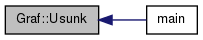
\includegraphics[width=224pt]{class_graf_a989e232821c5f0fa37d993168d56be6f_icgraph}
\end{center}
\end{figure}


\hypertarget{class_graf_a9c8c9ffa7ad533e0b5ab71d9addbaab5}{\index{Graf@{Graf}!Usunw@{Usunw}}
\index{Usunw@{Usunw}!Graf@{Graf}}
\subsubsection[{Usunw}]{\setlength{\rightskip}{0pt plus 5cm}void Graf\-::\-Usunw (
\begin{DoxyParamCaption}
\item[{int}]{wierzcholek}
\end{DoxyParamCaption}
)}}\label{class_graf_a9c8c9ffa7ad533e0b5ab71d9addbaab5}


Definicja w linii 38 pliku Graf.\-cpp.

\hypertarget{class_graf_a8340cd1321426d1a49b5e50f1c7e10f1}{\index{Graf@{Graf}!Visit\-Node@{Visit\-Node}}
\index{Visit\-Node@{Visit\-Node}!Graf@{Graf}}
\subsubsection[{Visit\-Node}]{\setlength{\rightskip}{0pt plus 5cm}void Graf\-::\-Visit\-Node (
\begin{DoxyParamCaption}
\item[{int}]{wierzcholek}
\end{DoxyParamCaption}
)}}\label{class_graf_a8340cd1321426d1a49b5e50f1c7e10f1}


Definicja w linii 80 pliku Graf.\-cpp.



Oto graf wywoływań tej funkcji\-:\nopagebreak
\begin{figure}[H]
\begin{center}
\leavevmode
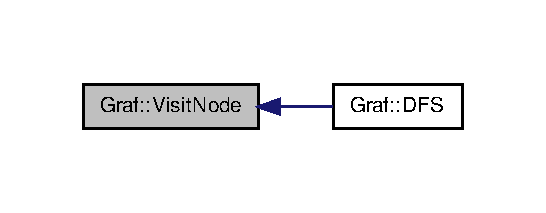
\includegraphics[width=262pt]{class_graf_a8340cd1321426d1a49b5e50f1c7e10f1_icgraph}
\end{center}
\end{figure}




\subsection{Dokumentacja atrybutów składowych}
\hypertarget{class_graf_a8cc46484cf7f96ce274d87829bf10120}{\index{Graf@{Graf}!colour@{colour}}
\index{colour@{colour}!Graf@{Graf}}
\subsubsection[{colour}]{\setlength{\rightskip}{0pt plus 5cm}vector$<$int$>$ Graf\-::colour}}\label{class_graf_a8cc46484cf7f96ce274d87829bf10120}


Definicja w linii 35 pliku Graf.\-h.

\hypertarget{class_graf_a72ccd052ab732941488da20d198aa82c}{\index{Graf@{Graf}!wektor@{wektor}}
\index{wektor@{wektor}!Graf@{Graf}}
\subsubsection[{wektor}]{\setlength{\rightskip}{0pt plus 5cm}vector$<$list$<${\bf para}$>$ $>$ Graf\-::wektor}}\label{class_graf_a72ccd052ab732941488da20d198aa82c}


Definicja w linii 39 pliku Graf.\-h.



Dokumentacja dla tej klasy została wygenerowana z plików\-:\begin{DoxyCompactItemize}
\item 
\hyperlink{_graf_8h}{Graf.\-h}\item 
\hyperlink{_graf_8cpp}{Graf.\-cpp}\end{DoxyCompactItemize}

\hypertarget{classpara}{\section{Dokumentacja klasy para}
\label{classpara}\index{para@{para}}
}


Modeluje pojęcie para. Klasa modeluje pojęcie para . Jej atrybutem sa pola zawierajace numer wierzcholka i jego wage.  




{\ttfamily \#include $<$para.\-h$>$}

\subsection*{Metody publiczne}
\begin{DoxyCompactItemize}
\item 
\hyperlink{classpara_ad30c7566519da720cef8f4ebf68b2e48}{para} ()
\begin{DoxyCompactList}\small\item\em Definicja konstruktora. \end{DoxyCompactList}\item 
virtual \hyperlink{classpara_ab6157584ffc475598c972a6563b5e1d5}{$\sim$para} ()
\begin{DoxyCompactList}\small\item\em Definicja konstruktora wirtualnego. \end{DoxyCompactList}\item 
\hyperlink{classpara_a12765ab1f150bcd071ce65ab2fee5acf}{para} (int \-\_\-waga, int \-\_\-numer)
\begin{DoxyCompactList}\small\item\em Inicjalizuje konstruktor. \end{DoxyCompactList}\end{DoxyCompactItemize}
\subsection*{Atrybuty publiczne}
\begin{DoxyCompactItemize}
\item 
double \hyperlink{classpara_abb3c97517be3143adbe2015fe69e3263}{G}
\begin{DoxyCompactList}\small\item\em Pomocnicza zmienna okreslajaca funkcje G. \end{DoxyCompactList}\item 
double \hyperlink{classpara_acf26fcfec428d059398ebc1b50f86ba8}{F}
\begin{DoxyCompactList}\small\item\em Pomocnicza zmienna okreslajaca funkcje F(suma funkcji G i H). \end{DoxyCompactList}\item 
double \hyperlink{classpara_aa042f1889262d8c7f34c50f1e0584086}{H}
\begin{DoxyCompactList}\small\item\em Pomocnicza zmienna okreslajaca funkcje H. \end{DoxyCompactList}\item 
int \hyperlink{classpara_a6ccf50eedaaef6b86ec2c051af6ccf8d}{waga}
\begin{DoxyCompactList}\small\item\em Zmienna zawierajace wage wierzcholka. \end{DoxyCompactList}\item 
int \hyperlink{classpara_ad00013e542cdbfd535beca41cb8d1e1f}{numer}
\begin{DoxyCompactList}\small\item\em Zmienna zawierajaca numer wierzcholka ktory jest sasiadem. \end{DoxyCompactList}\end{DoxyCompactItemize}


\subsection{Opis szczegółowy}


Definicja w linii 22 pliku para.\-h.



\subsection{Dokumentacja konstruktora i destruktora}
\hypertarget{classpara_ad30c7566519da720cef8f4ebf68b2e48}{\index{para@{para}!para@{para}}
\index{para@{para}!para@{para}}
\subsubsection[{para}]{\setlength{\rightskip}{0pt plus 5cm}para\-::para (
\begin{DoxyParamCaption}
{}
\end{DoxyParamCaption}
)}}\label{classpara_ad30c7566519da720cef8f4ebf68b2e48}


Definicja w linii 13 pliku para.\-cpp.

\hypertarget{classpara_ab6157584ffc475598c972a6563b5e1d5}{\index{para@{para}!$\sim$para@{$\sim$para}}
\index{$\sim$para@{$\sim$para}!para@{para}}
\subsubsection[{$\sim$para}]{\setlength{\rightskip}{0pt plus 5cm}para\-::$\sim$para (
\begin{DoxyParamCaption}
{}
\end{DoxyParamCaption}
)\hspace{0.3cm}{\ttfamily [virtual]}}}\label{classpara_ab6157584ffc475598c972a6563b5e1d5}


Definicja w linii 18 pliku para.\-cpp.

\hypertarget{classpara_a12765ab1f150bcd071ce65ab2fee5acf}{\index{para@{para}!para@{para}}
\index{para@{para}!para@{para}}
\subsubsection[{para}]{\setlength{\rightskip}{0pt plus 5cm}para\-::para (
\begin{DoxyParamCaption}
\item[{int}]{\-\_\-waga, }
\item[{int}]{\-\_\-numer}
\end{DoxyParamCaption}
)\hspace{0.3cm}{\ttfamily [inline]}}}\label{classpara_a12765ab1f150bcd071ce65ab2fee5acf}


Definicja w linii 55 pliku para.\-h.



\subsection{Dokumentacja atrybutów składowych}
\hypertarget{classpara_acf26fcfec428d059398ebc1b50f86ba8}{\index{para@{para}!F@{F}}
\index{F@{F}!para@{para}}
\subsubsection[{F}]{\setlength{\rightskip}{0pt plus 5cm}double para\-::\-F}}\label{classpara_acf26fcfec428d059398ebc1b50f86ba8}


Definicja w linii 31 pliku para.\-h.

\hypertarget{classpara_abb3c97517be3143adbe2015fe69e3263}{\index{para@{para}!G@{G}}
\index{G@{G}!para@{para}}
\subsubsection[{G}]{\setlength{\rightskip}{0pt plus 5cm}double para\-::\-G}}\label{classpara_abb3c97517be3143adbe2015fe69e3263}


Definicja w linii 27 pliku para.\-h.

\hypertarget{classpara_aa042f1889262d8c7f34c50f1e0584086}{\index{para@{para}!H@{H}}
\index{H@{H}!para@{para}}
\subsubsection[{H}]{\setlength{\rightskip}{0pt plus 5cm}double para\-::\-H}}\label{classpara_aa042f1889262d8c7f34c50f1e0584086}


Definicja w linii 35 pliku para.\-h.

\hypertarget{classpara_ad00013e542cdbfd535beca41cb8d1e1f}{\index{para@{para}!numer@{numer}}
\index{numer@{numer}!para@{para}}
\subsubsection[{numer}]{\setlength{\rightskip}{0pt plus 5cm}int para\-::numer}}\label{classpara_ad00013e542cdbfd535beca41cb8d1e1f}


Definicja w linii 51 pliku para.\-h.

\hypertarget{classpara_a6ccf50eedaaef6b86ec2c051af6ccf8d}{\index{para@{para}!waga@{waga}}
\index{waga@{waga}!para@{para}}
\subsubsection[{waga}]{\setlength{\rightskip}{0pt plus 5cm}int para\-::waga}}\label{classpara_a6ccf50eedaaef6b86ec2c051af6ccf8d}


Definicja w linii 47 pliku para.\-h.



Dokumentacja dla tej klasy została wygenerowana z plików\-:\begin{DoxyCompactItemize}
\item 
/home/karolina/\-Pulpit/astar/prj/\hyperlink{para_8h}{para.\-h}\item 
/home/karolina/\-Pulpit/astar/prj/\hyperlink{para_8cpp}{para.\-cpp}\end{DoxyCompactItemize}

\chapter{Dokumentacja plików}
\hypertarget{_graf_8cpp}{\section{Dokumentacja pliku Graf.\-cpp}
\label{_graf_8cpp}\index{Graf.\-cpp@{Graf.\-cpp}}
}


Funkcje do klasy \hyperlink{class_graf}{Graf}.  


{\ttfamily \#include \char`\"{}Graf.\-h\char`\"{}}\\*
Wykres zależności załączania dla Graf.\-cpp\-:\nopagebreak
\begin{figure}[H]
\begin{center}
\leavevmode
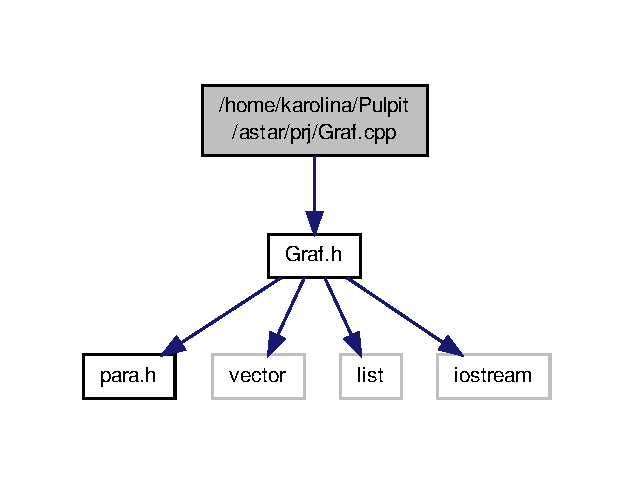
\includegraphics[width=304pt]{_graf_8cpp__incl}
\end{center}
\end{figure}

\hypertarget{_graf_8h}{\section{Dokumentacja pliku Graf.\-h}
\label{_graf_8h}\index{Graf.\-h@{Graf.\-h}}
}


Definicja klasy \hyperlink{class_graf}{Graf}.  


{\ttfamily \#include \char`\"{}para.\-h\char`\"{}}\\*
{\ttfamily \#include $<$vector$>$}\\*
{\ttfamily \#include $<$list$>$}\\*
{\ttfamily \#include $<$iostream$>$}\\*
Wykres zależności załączania dla Graf.\-h\-:\nopagebreak
\begin{figure}[H]
\begin{center}
\leavevmode
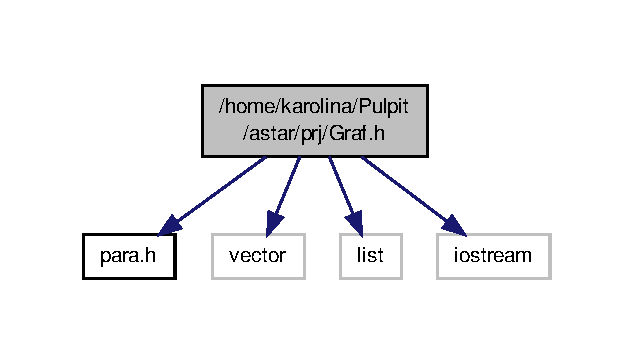
\includegraphics[width=304pt]{_graf_8h__incl}
\end{center}
\end{figure}
Ten wykres pokazuje, które pliki bezpośrednio lub pośrednio załączają ten plik\-:
\nopagebreak
\begin{figure}[H]
\begin{center}
\leavevmode
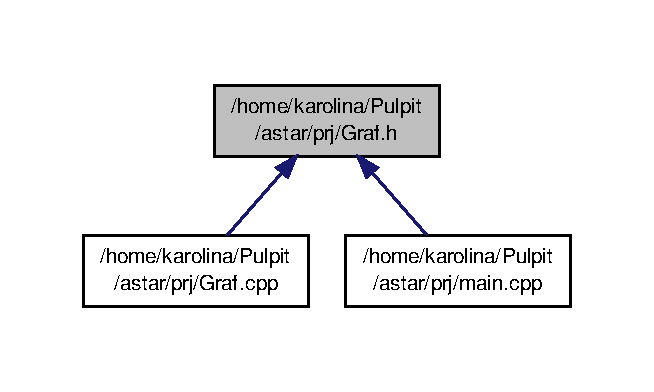
\includegraphics[width=208pt]{_graf_8h__dep__incl}
\end{center}
\end{figure}
\subsection*{Komponenty}
\begin{DoxyCompactItemize}
\item 
class \hyperlink{class_graf}{Graf}
\begin{DoxyCompactList}\small\item\em Modeluje pojęcie \hyperlink{class_graf}{Graf}. Klasa modeluje pojęcie graf . Jej atrybutem jest pole zawierajace liste sasedztwa. \end{DoxyCompactList}\end{DoxyCompactItemize}


\subsection{Opis szczegółowy}
Plik zawiera definicję klasy \hyperlink{class_graf}{Graf} Jest to klasa glowna , ktora wykorzystuje klase para. 

Definicja w pliku \hyperlink{_graf_8h_source}{Graf.\-h}.


\hypertarget{main_8cpp}{\section{Dokumentacja pliku /home/karolina/\-Pulpit/pamsi/prj/src/main.cpp}
\label{main_8cpp}\index{/home/karolina/\-Pulpit/pamsi/prj/src/main.\-cpp@{/home/karolina/\-Pulpit/pamsi/prj/src/main.\-cpp}}
}
{\ttfamily \#include $<$iostream$>$}\\*
{\ttfamily \#include $<$dzialania.\-hh$>$}\\*
{\ttfamily \#include $<$cstdlib$>$}\\*
Wykres zależności załączania dla main.\-cpp\-:
\subsection*{Funkcje}
\begin{DoxyCompactItemize}
\item 
int \hyperlink{main_8cpp_a3c04138a5bfe5d72780bb7e82a18e627}{main} (int argc, char $\ast$$\ast$argv)
\begin{DoxyCompactList}\small\item\em Funkcja main wykonuje algorytm i sprawdza czas dzialania algorytmu. W funkcji main wykonywane sa operacje \-: -\/\-Wczytywanie pliku z danymi wejsciowym -\/\-Dane sa mnozone razy 2 (w tej chwili wlaczany jest stoper) -\/\-Wczytywanie pliku z danymi sprawdzajacymi -\/\-Sprawdzanie zgodnosci -\/\-Stoper zostaje wylaczony i na wyjsciu programu podany zostaje czas dzialania algorytmu. \end{DoxyCompactList}\end{DoxyCompactItemize}


\subsection{Dokumentacja funkcji}
\hypertarget{main_8cpp_a3c04138a5bfe5d72780bb7e82a18e627}{\index{main.\-cpp@{main.\-cpp}!main@{main}}
\index{main@{main}!main.cpp@{main.\-cpp}}
\subsubsection[{main}]{\setlength{\rightskip}{0pt plus 5cm}int main (
\begin{DoxyParamCaption}
\item[{int}]{argc, }
\item[{char $\ast$$\ast$}]{argv}
\end{DoxyParamCaption}
)}}\label{main_8cpp_a3c04138a5bfe5d72780bb7e82a18e627}


Funkcja main wykonuje algorytm i sprawdza czas dzialania algorytmu. W funkcji main wykonywane sa operacje \-: -\/\-Wczytywanie pliku z danymi wejsciowym -\/\-Dane sa mnozone razy 2 (w tej chwili wlaczany jest stoper) -\/\-Wczytywanie pliku z danymi sprawdzajacymi -\/\-Sprawdzanie zgodnosci -\/\-Stoper zostaje wylaczony i na wyjsciu programu podany zostaje czas dzialania algorytmu. 



Definicja w linii 22 pliku main.\-cpp.


\hypertarget{para_8cpp}{\section{Dokumentacja pliku para.\-cpp}
\label{para_8cpp}\index{para.\-cpp@{para.\-cpp}}
}


Funkcje klasy para.  


{\ttfamily \#include \char`\"{}para.\-h\char`\"{}}\\*
Wykres zależności załączania dla para.\-cpp\-:\nopagebreak
\begin{figure}[H]
\begin{center}
\leavevmode
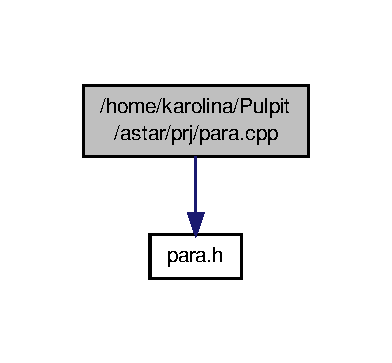
\includegraphics[width=134pt]{para_8cpp__incl}
\end{center}
\end{figure}

\hypertarget{para_8h}{\section{Dokumentacja pliku /home/karolina/\-Pulpit/astar/prj/para.h}
\label{para_8h}\index{/home/karolina/\-Pulpit/astar/prj/para.\-h@{/home/karolina/\-Pulpit/astar/prj/para.\-h}}
}


Definicja klasy para.  


Ten wykres pokazuje, które pliki bezpośrednio lub pośrednio załączają ten plik\-:
\nopagebreak
\begin{figure}[H]
\begin{center}
\leavevmode
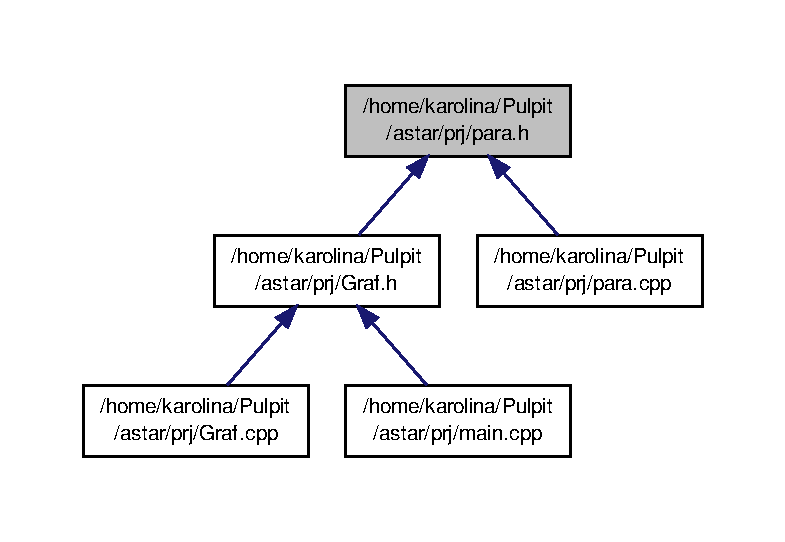
\includegraphics[width=350pt]{para_8h__dep__incl}
\end{center}
\end{figure}
\subsection*{Komponenty}
\begin{DoxyCompactItemize}
\item 
class \hyperlink{classpara}{para}
\begin{DoxyCompactList}\small\item\em Modeluje pojęcie para. Klasa modeluje pojęcie para . Jej atrybutem sa pola zawierajace numer wierzcholka i jego wage. \end{DoxyCompactList}\end{DoxyCompactItemize}


\subsection{Opis szczegółowy}
Plik zawiera definicję klasy para Jest to klasa pomocnicza wykorzystywana w klasie \hyperlink{class_graf}{Graf}. 

Definicja w pliku \hyperlink{para_8h_source}{para.\-h}.


\addcontentsline{toc}{part}{Indeks}
\printindex
\end{document}
